\documentclass[main.tex]{subfiles}
\begin{document}

\subsection{Назначение и принцип работы прибора}
Заданный курсовой прибор является гирополукомпасом, так как предназначен для отслеживания 
заданного азимута. Гирополукомпас (ГПК) – курсовой гироскопический прибор, построенный 
на основе трехстепенного астатического гироскопа, имеет системы горизонтальной и 
азимутальной коррекции. Кинематическая схема ГПК приведена на рисунке 1. Система 
горизонтальной коррекции состит из ЧЭ – датчика угла \( \text{ДУ}_1 \), расположенного по оси 
внутренней рамки гироскопа, и исполнительного элемента – электродвигателя ЭДВ, 
создающего момент относительно оси наружной рамки \( Oy_1 \). Базовая система 
координат \( O\xi\eta\zeta \) - географическая.\par

При отклонении вектора Н от плоскости горизонта на угол \( \beta \) на выходе \( \text{ДУ}_1 \)
 появляется напряжение \( U=K_\text{ДУ}\beta \) при \( \beta < \beta_\text{п} \). 
 ЭДВ при наличии тока создает момент \( M_\text{эдв}=E\beta \)относительно оси 
 наружной рамки \( Oy_1 \), из-за чего возникает прецессия гироскопа 
 \( \dot{\beta}=\frac{M_\text{эдв}}{H} = \frac{E\beta}{H} = \varepsilon\beta \). \par

Датчик момента ДМ азимутальной коррекции управляется напряжением, поступающим 
с пульта, и компенсирует величину \( \omega_\zeta \approx U\sin(\varphi) \). Момент ДМ
азимутальной коррекции \( M_{\text{ДМ}_2} \approx H\omega_\zeta = HU/sin(\varphi)\).
 Система азимутальной коррекции позволяет скомпенсировать постоянную 
 составляющую \( \omega_0 \) собственной скорости прецессии. Поэтому на пульте
  устанавливаются 2 потенциометра со шкалами \( \varphi \) (в градусах – широта), и 
  \( \omega_0 \) (гр/ч). Величину \( \omega_0 \) определяют по показаниям ГПК в сравнении
   с показаниями других средств (GPS, магнитный компас) на стоянке аэродрома 
   или в прямолинейном полете с постоянной линейной скоростью. Момент азимутальной 
   коррекции с учетом \( \omega_0 \): \( M_{\text{ДМ}_2} \approx H(U\sin(\varphi) + \omega_0 \). \par

ГПК предназначены для отслеживания азимута (заданного направления) и находят 
широкое применение в авиации и наземных объектах.

\begin{figure}[h]
\begin{minipage}[h]{0.49\linewidth}
    \center{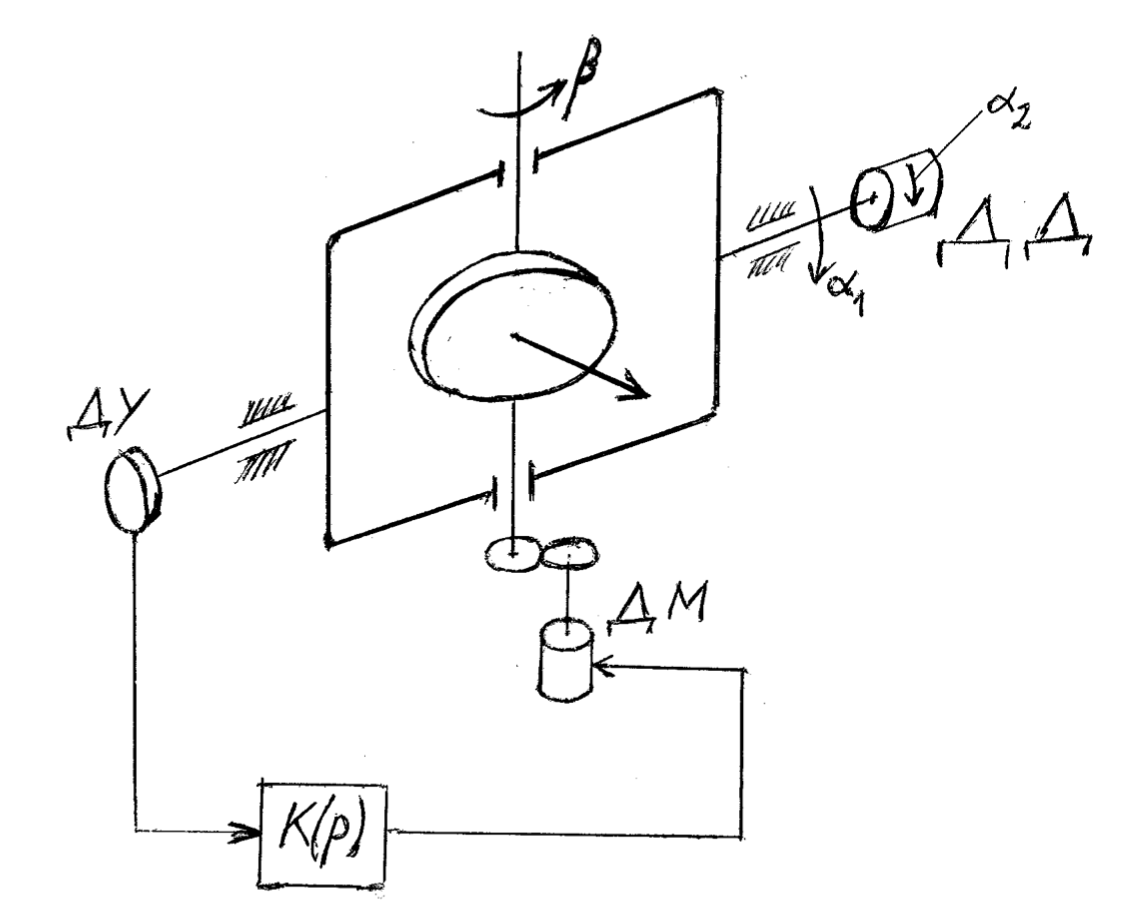
\includegraphics[width=1\linewidth]{images/p1_schema.png}}
    \caption{Общий вид системы}
\end{minipage}
\begin{minipage}[h]{0.49\linewidth}
    \center{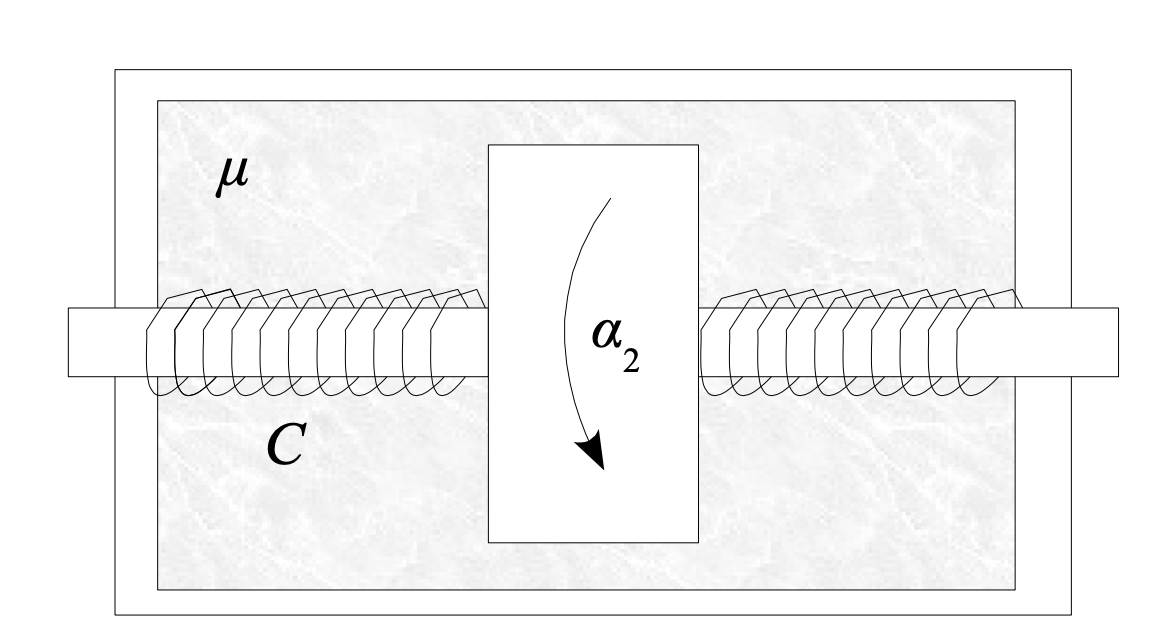
\includegraphics[width=1\linewidth]{images/p1_demfer.png}}
    \caption{Демпфер}
\end{minipage}
\end{figure}

\newcommand{\Mdd}{M_\text{ДД}}
\newcommand{\Koc}{K_\text{ОС}}
\newcommand{\Ad}{A_\text{д}}
\newcommand{\ad}{\alpha_\text{д}}

\subsection{Уравнения движения ГПК с соответствующей нелинейностью}
\begin{enumerate}
    \item Уравнение движения наружной рамки:
    \[ A\ddot{\alpha} +  \Mdd - H\dot{\beta} - \Koc\beta + \varphi(\dot{\alpha}) = M_\alpha\]

    \item Уравнение движения внутренней рамки
    \[ B\ddot{\beta} + \mu_\beta\dot{\beta} + H\dot{\alpha} = M_\beta \]

    \item Уравнение движения динамического демфера
    \[ \Ad\ddot{\ad} - \Mdd = M_{\ad} \]

    \item Момент динамического демфера
    \[ \Mdd = \mu(\dot{\alpha} - \dot{\ad}) + C(\alpha - \ad) \]
\end{enumerate}

\subsection{Расчёт выражения для передаточных функций гиросистемы как объекта управления и как объекта стабилизации}
    Запишем уравнения движения без учета трения в опорах (и, соответственно, нелинейности):
    \begin{equation}\begin{cases}
        A\ddot{\alpha} +  \mu(\dot{\alpha} - \dot{\ad}) + C(\alpha - \ad) 
            - H\dot{\beta} - \Koc\beta = M_\alpha, \\
        B\ddot{\beta} + H\dot{\alpha} = M_\beta, \\
        \Ad\ddot{\ad} - \mu(\dot{\alpha} - \dot{\ad}) - C(\alpha - \ad) = M_{\ad}
    \end{cases}\end{equation}

    Преобразуем систему уравнений по Лапласу:
    \begin{equation}\begin{cases}
        A\alpha s^2 + \mu s(\alpha - \ad) + C(\alpha - \ad) - H\beta s - \Koc\beta= M_\alpha, \\
        B\beta s^2 + H\alpha s = M_\beta, \\
        \Ad\ad s^2 - \mu s(\alpha - \ad) - C(\alpha - \ad) = M_{\ad},
    \end{cases}\end{equation}

    и запишем в векторно-матричной форме:
    \[
    \begin{bmatrix}
        As^2 + \mu s + C & -Hs - \Koc & -\mu s - C \\
        Hs & Bs^2 & 0 \\
        -\mu s - C & 0 & \Ad s^2 + \mu s + C \\
    \end{bmatrix} \begin{bmatrix}\alpha \\ \beta \\ \ad\end{bmatrix} = 
    \begin{bmatrix}M_{\alpha} \\ M_{\beta} \\ M_{\ad} \\ \end{bmatrix}.
    \]
    
    Разрешим полученную систему уравнений относительно вектора 
    \( \begin{bmatrix} \alpha & \beta & \ad \end{bmatrix}^T\):

    \[
    \begin{bmatrix}\alpha \\ \beta \\ \ad\end{bmatrix} = 
    \begin{bmatrix}
        W^{\alpha}_{M_{\alpha}} & W^{\alpha}_{M_{\beta}} & W^{\alpha}_{M_{\ad}} \\
        W^{\beta}_{M_{\alpha}} & W^{\beta}_{M_{\beta}} & W^{\beta}_{M_{\ad}} \\
        W^{\ad}_{M_{\alpha}} & W^{\ad}_{M_{\beta}} & W^{\ad}_{M_{\ad}} \\
    \end{bmatrix} \begin{bmatrix}M_{\alpha} \\ M_{\beta} \\ M_{\ad}\end{bmatrix}.
    \]

    Заметим, что искомая матрица передаточных функций - ни что иное как 
    обратная матрица системы уравнений. Получимеё с помощью возможностей символьного 
    вычисления Matlab. Для дальнейшей работы необходимы лишь две передаточных функции,
    их и запишем:
    \begin{enumerate}
        \item системы как объекта управления
            \[ W^{\beta}_{M_{\alpha}} = \frac{-H(\Ad s^2 + \mu s + C)}{\Delta}, \]

        \item системы как объекта стабилизации
            \[ W^{\alpha}_{M_{\alpha}} = \frac{Bs(\Ad s^2 + \mu s + C)}{\Delta}, \]        
    \end{enumerate}
    Здесь \( \Delta \) - определитель матрицы системы (после сокращения одной s):
    \[ \Delta = A\Ad B s^5 + \mu B(A+\Ad)s^4 + (\Ad H^2+BC(A+\Ad))s^3 + \] 
        \[+ H(\Ad\Koc+H\mu)s^2 + H(CH+\Koc\mu)s + CH\Koc. \] \par
    Получили передаточные функции системы как объекта управления и объекта стабилизации
    в общем виде.

\subsection{Оптимизация параметров упруго-диссипативной связи динамических 
элементов гиросистемы по критерию \( minmax |W(j\omega)| \)}

    Проведём оптимизацию параметров \( \mu \) и C для ДД. Для этого рассмотрим разомкнутую
    ПФ курсового гироскопа как объекта стабилизации (принимаем \( \Koc=0 \)).\par 

    Запишем полное выражение вышеназванной ПФ с указанными допущениями:
    \begin{equation}\label{eq:KJLDwdI}
    W^{\alpha}_{M_{\alpha}} = \frac{
        Bs(\Ad s^2 + \mu s + C)
    }{
        A\Ad B s^5 + \mu B(A+\Ad)s^4 + (\Ad H^2+BC(A+\Ad))s^3 + H^2\mu s^2 + CH^2s
    }
    \end{equation}

    Эта ПФ обладает замечательным свойством: при одном значении C, но разных \( \mu \), на АЧХ 
    будут существовать две инвариантные точки (все АЧХ пересекаются в них). При изменении С эти 
    точки будут перемещаться. \par 

    Целью оптимизации является минимизация максимумов АЧХ ПФ, а именно минимизация резонансных 
    пиков АЧХ. Таким образом, учитывая особенности нашей ПФ, оптимизация сводится к следующим
    двум этапам:
    \begin{itemize}
        \item Поиск значения \( C^* \), при котором инвариантные точки будут располагаться 
        на одном уровне, тем самым обеспечивается минимальное значение амплитуды в обеих инвариантных точках;
        \item Поиск значения \( \mu^* \), обеспечивающего минимальное значение резонансных пиков.
    \end{itemize}

\subsubsection*{Поиск значения \( C^* \)}
    Условие инвариантности имеет следующий вид:
    \[ |W(j\omega)|_{\mu=0} = |W(j\omega)|_{\mu=\infty} \]
    После раскрытия модуля получаем:
    \[ W(j\omega)_{\mu=0} = -W(j\omega)_{\mu=\infty}\]
    
    С помощью Matlab вычислим пределы:
    \[ \frac{
        B(\Ad(j\omega)^2 + C)
    }{
        A\Ad B (j\omega)^4 + (\Ad H^2+BC(A+\Ad))(j\omega)^2
    } = \frac{-B}{B(A+\Ad)(j\omega)^2 + H^2} \]
    \begin{equation}\label{eqn:W}
    \frac{ B(\Ad\omega^2 - C) }{
        A\Ad B\omega^4 - (\Ad H^2+BC(A+\Ad))\omega^2 + CH^2
    } = \frac{B}{H^2  - B(A+\Ad)\omega^2}
    \end{equation}
    
    Решаем уравнение относительно C. В результате получаем четыре корня. Два из них отрицательные и не 
    удовлетворяют ОДЗ. Два других же вполне соответствуют инвариантным точкам \( \omega_1 \) и \( \omega_2 \):
    \[ \omega_{1,2} = \sqrt{\frac{
        \Ad H^2 + BC(A + \Ad) \pm \sqrt{B^2C^2(A^2+\Ad^2) + 2A\Ad BC^2 - 2A\Ad BCH^2 + \Ad^2H^4}
    }{\Ad B(2A + \Ad)}} \]

    Подставив численные значения, получаем следующие функции:
    \[ \omega_{1,2} = \sqrt{\frac{
        10^6 + 0,6C \pm \sqrt{0,36C^2 - 10^6C + 10^{12}}
    }{11}} \]

    Известно, что в инвариантных точках значения амплитуд равны, что
    можно записать как
     \[ | W(j\omega) |^{\omega=\omega_1}_{\mu=0}  = | W(j\omega) |^{\omega=\omega_2}_{\mu=0} \]
    
     Подставим сюда ПФ из правой части (\ref{eqn:W}) и раскроем модуль:
    \begin{equation}\label{eq:1Mdb}\begin{multlined}
        \frac{ B(\Ad\omega_1^2 - C) }{
        A\Ad B\omega_1^4 - (\Ad H^2+BC(A+\Ad))\omega_1^2 + CH^2
    } = \\ = \frac{ B(\Ad\omega_2^2 - C) }{
        A\Ad B\omega_2^4 - (\Ad H^2+BC(A+\Ad))\omega_2^2 + CH^2
    }
    \end{multlined}\end{equation}

    Имея значения частот от C, решим уравнение (\ref{eq:1Mdb}) относительно С. \par 
    Получаем \( C^* = \frac{12500000}{9} \approx 13,89\cdot 10^5 \).
    
    С учетом полученного значения рассчитаем \( \omega_1,\ \omega_2 \): \\
    \begin{tabular}{p{0.2\linewidth}p{0.3\linewidth}p{0.4\linewidth}}
        & \( \omega_1 = 465,5 \) & \( \omega_2 = 341,2 \) \\
        & \( lg \omega_1 = 2,668 \) & \( lg \omega_2 = 2,53 \) \\
    \end{tabular}

    \begin{figure}[h]
        \center{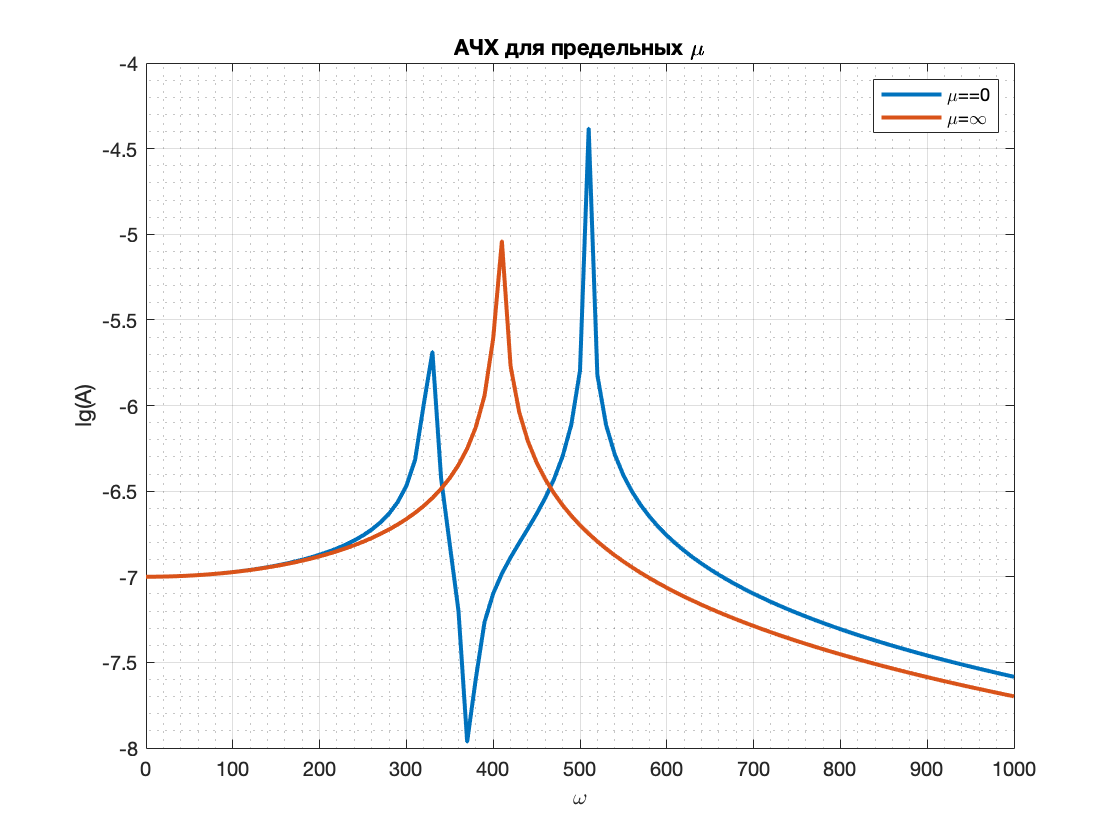
\includegraphics[width=1\linewidth]{images/p4_extremalbode.png}}
        \caption{АЧХ системы для оптимального C* и предельных \( \mu \)}
    \end{figure}

\subsubsection*{Поиск значения \( \mu^* \)}
    Для определения значения \( \mu^* \) следует определить значения \( \mu_1 \) и \( \mu_2 \), 
    при которых в каждой из инвариантных точек будет экстремум АЧХ (это
    обеспечивает минимум «всплеска» АЧХ в соответствующих инвариантных
    точках). Тогда 
     \[ \mu^* = \frac{\mu_1 + \mu_2 }{2} \]

    Запишем условия поиска:
    \begin{equation}\begin{cases}
        \frac{\partial |W(J\omega)|}{\partial\omega} \rvert_{\omega=\omega_1} = 0, \\
        \frac{\partial |W(J\omega)|}{\partial\omega} \rvert_{\omega=\omega_2} = 0
    \end{cases}\end{equation}

    \[ W(j\omega) = \frac{M(j\omega)}{N(J\omega)}, \]
    где 
    \begin{equation}\begin{cases}
        M(j\omega) = B(\Ad (j\omega)^2 + \mu (j\omega) + C), \\
        N(J\omega) = A\Ad B (j\omega)^4 + \mu B(A+\Ad)(j\omega)^3 + \\
        + (\Ad H^2+BC(A+\Ad))(j\omega)^2  + H^2\mu j\omega + CH^2
    \end{cases}\end{equation}

    \begin{equation}\begin{cases}
        M(j\omega) = B( - \Ad \omega^2 + j\mu\omega + C), \\
        N(J\omega) = A\Ad B \omega^4 -\mu B(A+\Ad)j\omega^3 - \\
        - (\Ad H^2+BC(A+\Ad))\omega^2  + H^2\mu j\omega + CH^2
    \end{cases}\end{equation}

    Для каждого \( \omega \) решим уравнение. Получим:
    \begin{equation}\begin{cases}
        \mu_1= 1767,26 \\
        \mu_2=1954,77 \\
    \end{cases}\end{equation}
    Тогда \( \mu^*=1861,01 \). \par

    Построим АЧХ для этого значения (см рис. \ref{fig:optimal_bode}).


\subsection{АЧХ механической части гиросистемы с оптимальными параметрами \( \mu \) и С}
    Построим АЧХ системы на основе функции (\ref{eq:KJLDwdI}), 
    куда подставим найденные оптимальные параметры (см рис. \ref{fig:optimal_bode}).

    \begin{figure}[h]
        \center{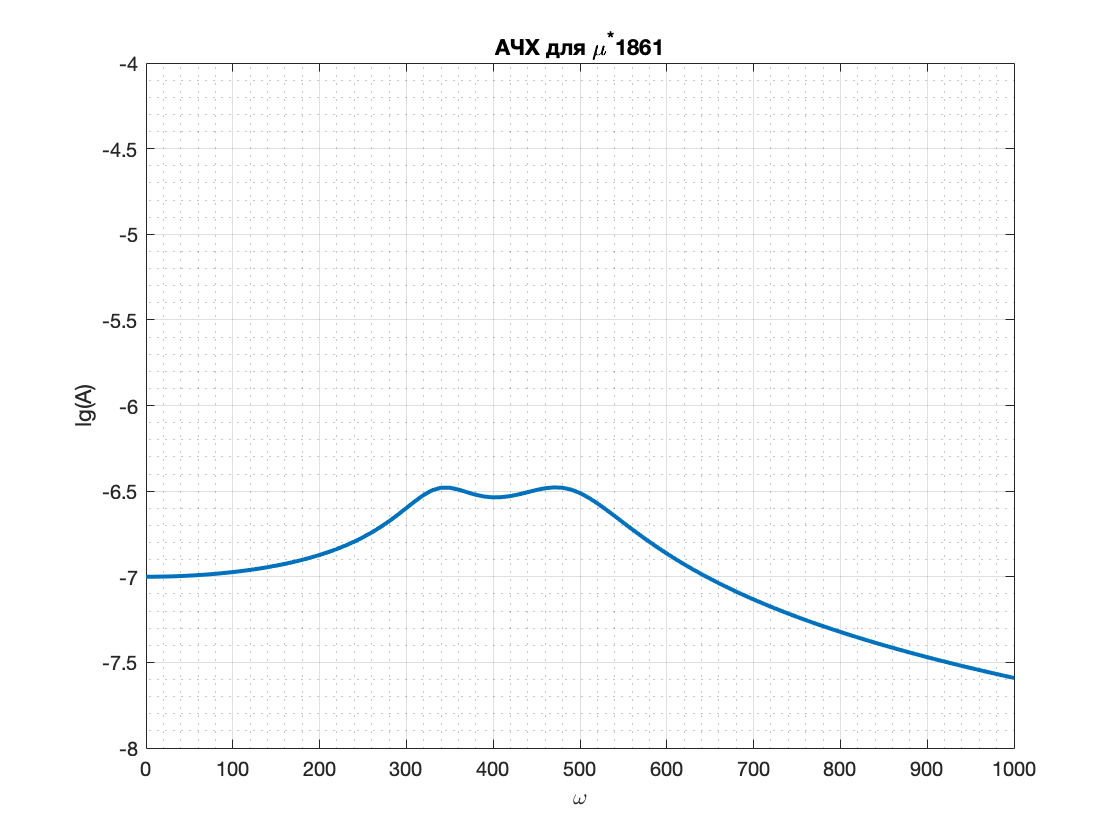
\includegraphics[width=1\linewidth]{images/p4_optimalbode.png}}
        \caption{АЧХ системы для оптимальных C* и \( \mu^* \)}
        \label{fig:optimal_bode}
    \end{figure}
\end{document}